Predictions were conducted for an idealized wind state to assess the generalization of the identified models. The idealized wind state is a simplified hydrodynamic condition where the models have a drift angle but no yaw rate or rudder angle. This is meant to represent a state in which the ship experiences a static drift angle for an extended period that is induced by a side wind force.
\autoref{fig:result_wind_state} shows the prediction results for the idealized wind condition. The sway force $Y_D$ of the PI model is very similar to that of the reference model. For the PU model, the sway force seems to be too large. The yawing moment $N_D$ is under-predicted by both models, but the difference is more significant for the PU model because most of the yawing moment is attributed to the yaw rate coefficients (as stated in the previous section), which are not activated in the wind state. 
The PI model seems to have a split between the yaw rate-- and drift angle--dependent coefficients in a more similar way to the more physically correct reference model.
\label{sec:wind_state}
\begin{figure}[h!]
    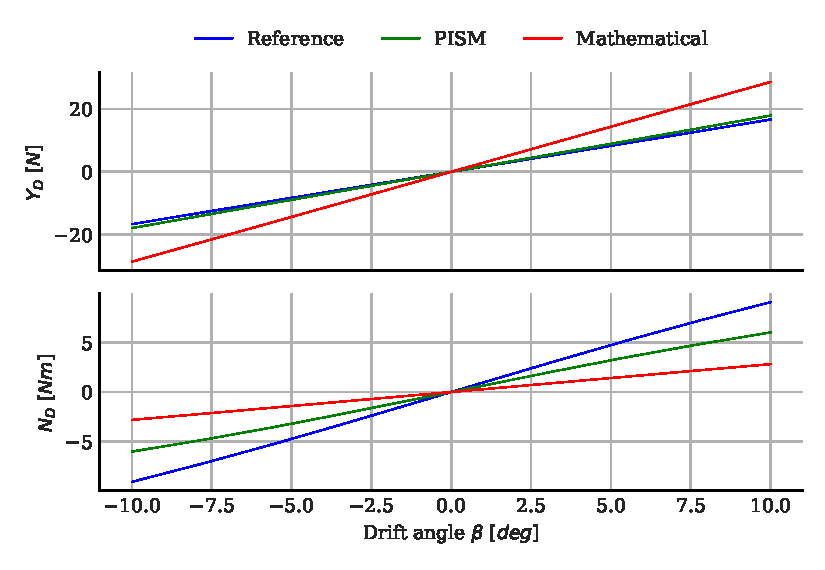
\includegraphics{figures/result_wind_state.forces.pdf}
    \caption{Total sway force and yawing moment from the wPCC models at various drift angles.}
    \label{fig:result_wind_state}
\end{figure}